%        File: network.tex
%     Created: Thu Jun 14 02:00 PM 2012 E
% Last Change: Thu Jun 14 02:00 PM 2012 E
%
\documentclass{article}

\usepackage{fullpage,amsmath,multicol,enumitem,graphicx,float,tikz}
\usepackage[T1]{fontenc}

\usetikzlibrary{decorations.pathreplacing,decorations.pathmorphing}

\title{Notes for Spring Network Simulator}
\author{Miles Yucht}
\date{\today}

\begin{document}
\maketitle
\hrule
\begin{multicols}{2}
    \section{Theory}
    
    \begin{figure}[H]
        \centering
        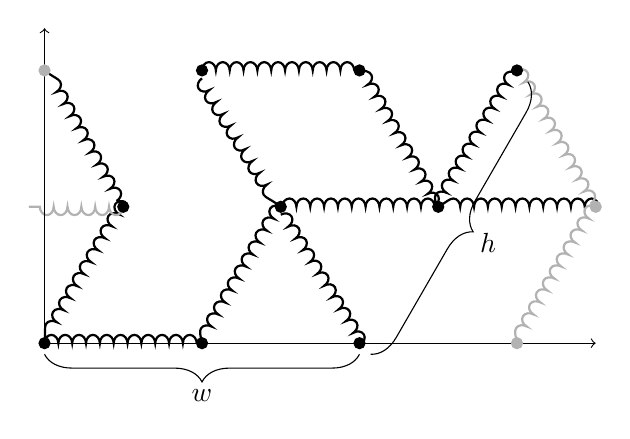
\begin{tikzpicture}
            \draw [thick,decorate,decoration={bumps,aspect=0.3,amplitude=3}] ( 0,0 ) -- ( 1.8,0 )
                    ( 0,0 ) -- ( 1, 1.732051 )
                    ( 2,0 ) -- ( 3,1.732051 )
                    ( 3,1.632051 ) -- ( 4,0 )
                    ( 3,1.732051 ) -- ( 4.8,1.732051 )
                    ( 3,1.732051 ) -- ( 2,3.364102 )
                    ( 2,3.464102 ) -- ( 3.9,3.464102 )
                    ( 4,3.464102 ) -- ( 4.9,1.832051 )
                    ( 5,1.732051 ) -- ( 6.9,1.732051 )
                    ( 0,3.464102 ) -- ( 0.9, 1.832051 )
                    ( 5,1.732051 ) -- ( 6,3.464102 );
            \draw [thick,decorate,decoration={bumps,aspect=0.3,amplitude=3},gray!60!white] 
                    ( 6,3.464102 ) -- ( 6.9,1.832051 )
                    ( 6, 0 ) -- ( 7,1.732051 )
                    ( 1,1.732051 ) -- ( -0.2,1.732051 );
            \draw[->] ( 0, 0 ) -- ( 0, 4 );
            \draw[->] ( 0, 0 ) -- ( 7, 0 );
            \filldraw [black] ( 0,0 ) circle ( 2pt )
                              ( 2,0 ) circle ( 2pt )
                              ( 4,0 ) circle ( 2pt )
                              ( 1,1.732051 ) circle ( 2pt )
                              ( 3,1.732051 ) circle ( 2pt )
                              ( 5,1.732051 ) circle ( 2pt )
                              ( 2,3.464102 ) circle ( 2pt )
                              ( 4,3.464102 ) circle ( 2pt )
                              ( 6,3.464102 ) circle ( 2pt );
            \filldraw [gray!60!white] ( 0,3.464102 ) circle ( 2pt )
                             ( 6, 0 ) circle ( 2pt )
                             ( 7,1.732051 ) circle ( 2pt );
            \draw [decorate,decoration={brace,amplitude=10pt,mirror,raise=-4pt},xshift=0pt,yshift=-8pt] ( 0,0 ) -- ( 4,0 ) node
                             [black,midway,yshift=-11pt] {$ w $};
            \draw [decorate,decoration={brace,amplitude=10pt,mirror},xshift=4pt,yshift=-4pt] ( 4,0 ) -- ( 6,3.464102 ) node
                             [black,midway,yshift=-9pt,xshift=14pt] {$ h $};
        \end{tikzpicture}
        \label{fig:lattice}
        \caption{\small This figure shows a sample lattice representing the network that was used in the simulation. The size of the lattice is $ w \times h
        $; in this case, it is $ 3 \times 3 $. Each coil represents a simulated bond, modeled as a Hookean spring. Black springs and nodes are
        considered to be in one network, and gray ones represent the periodic boundary conditions imposed on the system.}
    \end{figure}

    In the node network model, nodes are arranged into a finite equilateral triangular lattice. The distance between any neighboring nodes on such a
    network is the same. In our model, this distance is stored as $ \ell_{0} $, a constant representing the resting spring length. Between any
    neighboring nodes, there is a probability $ p $ of finding a spring there; this is equivalent to a spring with a Young's modulus of $ 0 $, so
    there is no energy penalty for deforming it.
    
    In the data structure, each Node object has three fields: first, an array of the xy-position of the node, with respect to the initial position of
    the first node; second, the stiffness of the three springs connected to the Node, and lastly a field for the resting length of the spring. The
    energy of the system is calculated using the following equation:

    \begin{equation}
        E_{total} = \frac{1}{2\ell_{0}} \sum\limits_{i}^{h} \sum\limits_{j}^w \sum\limits_{k=1}^3 \mu_{ij,k}( \delta \ell_{ij,k} )^2
        \label{eqn:energy}
    \end{equation}
    
    Here, $ \mu_{ij,k} $ is the spring constant between the Node at index $ ( i,j ) $ and that at index $ k $, where

    \begin{align*}
        k & = 1 \to ( i, j+1 ) \\
        k & = 2 \to ( i+1, j ) \\
        k & = 3 \to ( i+1, j-1 )
    \end{align*}
    
    Periodic boundary conditions are imposed so that, when $ i = h $ and $ j = w $ or $ j = 0 $, the Node at index $ k $ will actually refer to the
    node on the opposide edge of the network transposed by the height or width of the network.
    
    With no strain on the system, all springs remain at their rest length, and the energy of the system is 0. To create a strain on the system, we
    imposed Lees-Edwards boundary conditions by adding a factor $ x_{adj} $ of the strain $ \gamma $ times $ \ell_{0} $ to the x-coordinate of nodes $
    k = 2 $ and $ k = 3 $ when $ i = h $. Because of the periodicity of the system, this twists the entire network, increasing the energy of the
    system from 0 to a finite value depending on the strain, Young's modulus of the springs, the rest length of a spring, and the size of the network.

    \section{File Hierarchy}
    
    There are 8 header files and one main file in this project.

    \section{File Details}
    


\end{multicols}
\end{document}


